\cleardoublepage                                   
\chapter{Agente de Carga (AC)}

\section{Hardware}

%---------------------------------------descripción general del hardware---------------------------------------
El AC está implementado sobre una placa de desarrollo basada en un microcontrolador ESP32 de 32 bits. La elección de esta plataforma responde a su adecuada capacidad de procesamiento e interfaces para las tareas requeridas, su amplia disponibilidad en el mercado junto a un bajo costo y la extensa base de recursos técnicos existentes, lo que facilita su programación y mantenimiento. Este dispositivo integra las funciones de adquisición de datos, cálculo de variables eléctricas y comunicación tanto con la microrred como con los NC.

El sistema cuenta en primer lugar con una etapa de alimentación encargada de acondicionar la tensión de corriente alterna proveniente de la microrred para energizar el circuito completo. La estabilidad de esta fuente es fundamental, ya que variaciones significativas en su salida introducen errores en las mediciones realizadas por el AC o pueden afectar el desempeño del microcontrolador.

Para la medición de la tensión de la microrred se emplea un módulo sensor basado en el transformador de señal ZMPT101B, seleccionado tanto por sus características técnicas como por su disponibilidad comercial. Este módulo genera una señal sinusoidal con un nivel de continua (offset) y una amplitud proporcional a la tensión real medida. Antes de ser leída por la entrada analógica del microcontrolador, la señal atraviesa una etapa de adecuación que garantiza que sus valores se mantengan dentro del rango permitido por el ESP32, evitando sobrepasar el límite máximo de 3,3 V.

Con el fin de comunicarse con los demás agentes que intervienen en la microrred, el AC incorpora un módulo CAN basado en el controlador MCP2515. Este dispositivo actúa como interfaz física entre el microcontrolador y el bus diferencial del protocolo CAN, permitiendo tanto el envío como la recepción de mensajes. El módulo se conecta al ESP32 mediante la interfaz SPI, a través de la cual se gestionan las señales de control (CS, INT) asociadas a la transmisión y recepción de datos.

El intercambio de información entre el AC y los NC se complementa mediante el protocolo inalámbrico ESP-NOW, soportado nativamente por el ESP32. Este protocolo opera en la banda Wi-Fi pero utiliza directamente la capa de enlace de datos. Al prescindir de redes Wi-Fi existentes, encabezados adicionales y procesos de reensamblado, ofrece baja latencia y alta confiabilidad en enlaces de corto a mediano alcance.

En virtud de la naturaleza distribuida del sistema, el AC también actúa como receptor de los datos de consumo enviados por todos los NC. Estos valores, junto con los parámetros globales de consumo y generación de la microrred que el propio AC calcula, son transmitidos mediante una interfaz UART a un módulo ESP32-S3 Super Mini. Este módulo tiene como función publicar la información recibida en un servidor externo para su almacenamiento, visualización y análisis posterior, permitiendo así integrar la operación local de la microrred con herramientas remotas de supervisión.

Finalmente, el AC incorpora una interfaz local destinada a la interacción con el usuario. Esta incluye un display que proporciona retroalimentación visual inmediata y que se comunica con el microcontrolador mediante la interfaz serie I²C. Se integran además pulsadores que permiten navegar entre distintas pantallas e ingresar parámetros operativos del Sistema de Gestión de Consumo (SGC), facilitando su configuración y supervisión sin necesidad de herramientas externas.

%---------------------------------------descripción del diseño PCB---------------------------------------
Pensando en la integración del AC dentro de instalaciones eléctricas ya existentes, se consideró fundamental que su montaje no requiriera intervenciones complejas ni modificaciones significativas de la infraestructura del usuario. En entornos residenciales, comerciales e industriales es habitual la presencia de cajas de paso estandarizadas de 10×10 cm, ampliamente utilizadas en canalizaciones eléctricas convencionales. Con el fin de favorecer la compatibilidad con este tipo de cajas y facilitar su incorporación por parte de instaladores de sistemas de microrredes, el diseño de la placa de circuito impreso (PCB) del AC se desarrolló teniendo en cuenta esta restricción dimensional desde el inicio del proceso.

La PCB se definió para ajustarse al espacio interno de la caja mencionada, respetando las distancias necesarias para acomodar todos los componentes que forman parte del circuito, la separación entre zonas de baja tensión y las partes asociadas a la medición de la tensión del bus y la fuente de alimentación. En base a estas consideraciones se organizaron los componentes siguiendo una disposición que permitiera mantener recorridos cortos en la medida de lo posible para las señales sensibles como, por ejemplo, la adquisición de la tensión, asegurar una correcta disipación térmica y reservar ubicaciones accesibles para conectores, borneras y elementos de interfaz con el usuario.

El diseño final del PCB, mostrado en la Figura X, refleja estas decisiones, integrando en un espacio compacto todos los elementos funcionales del AC y permitiendo su instalación en una caja de paso estándar sin requerir adaptadores adicionales. Esta compatibilidad busca facilitar significativamente su implementación, reduciendo tiempos y costos de instalación y contribuyendo a que el sistema pueda ser incorporado como un módulo más dentro de las soluciones habituales manejadas por empresas instaladoras de sistemas de paneles solares.

%---------------------------------------imagen del diseñoPCB--------------------------------------

%---------------------------------------descripción del armado---------------------------------------
En cuanto al proceso de fabricación del prototipo, el mismo se realizó en base técnicas accesibles que permitieran validar el funcionamiento del AC antes de avanzar hacia una producción más estandarizada. La PCB fue elaborada mediante el método de transferencia, técnica ampliamente utilizada en etapas iniciales de desarrollo por su bajo costo y rapidez de implementación. Una vez transferido el diseño al cobre y completado el proceso de grabado mediante la reacción química de oxidación-reducción con cloruro férrico, se realizaron las perforaciones necesarias para la colocación de los componentes, conectores y módulos externos. Posteriormente, se llevó a cabo el montaje y la soldadura de todos los elementos, asegurando una correcta fijación mecánica y verificando la continuidad eléctrica en cada etapa.

Con el objetivo de integrar la interfaz local en la caja de paso de 10×10 cm, se efectuó un mecanizado de la tapa para alojar tanto los pulsadores como el display. La disposición de estos elementos fue seleccionada para garantizar accesibilidad al usuario, buena visibilidad y comodidad durante la utilización del sistema. Para asegurar un montaje firme y estético del display, se diseñó un soporte específico mediante software de modelado tridimensional y se imprimió en 3D utilizando material plástico de alta resistencia. Este soporte permite fijar el display en la posición adecuada y facilita el ensamblaje final sin necesidad de herramientas adicionales.

El conjunto resultante, mostrado en la Figura~\ref{img:ac}, combina una PCB que cumple con las restricciones de diseño y una interfaz accesible en un dispositivo práctico para la instalación en una infraestructura existente.


\begin{figure}[hbt!]
    \centering
    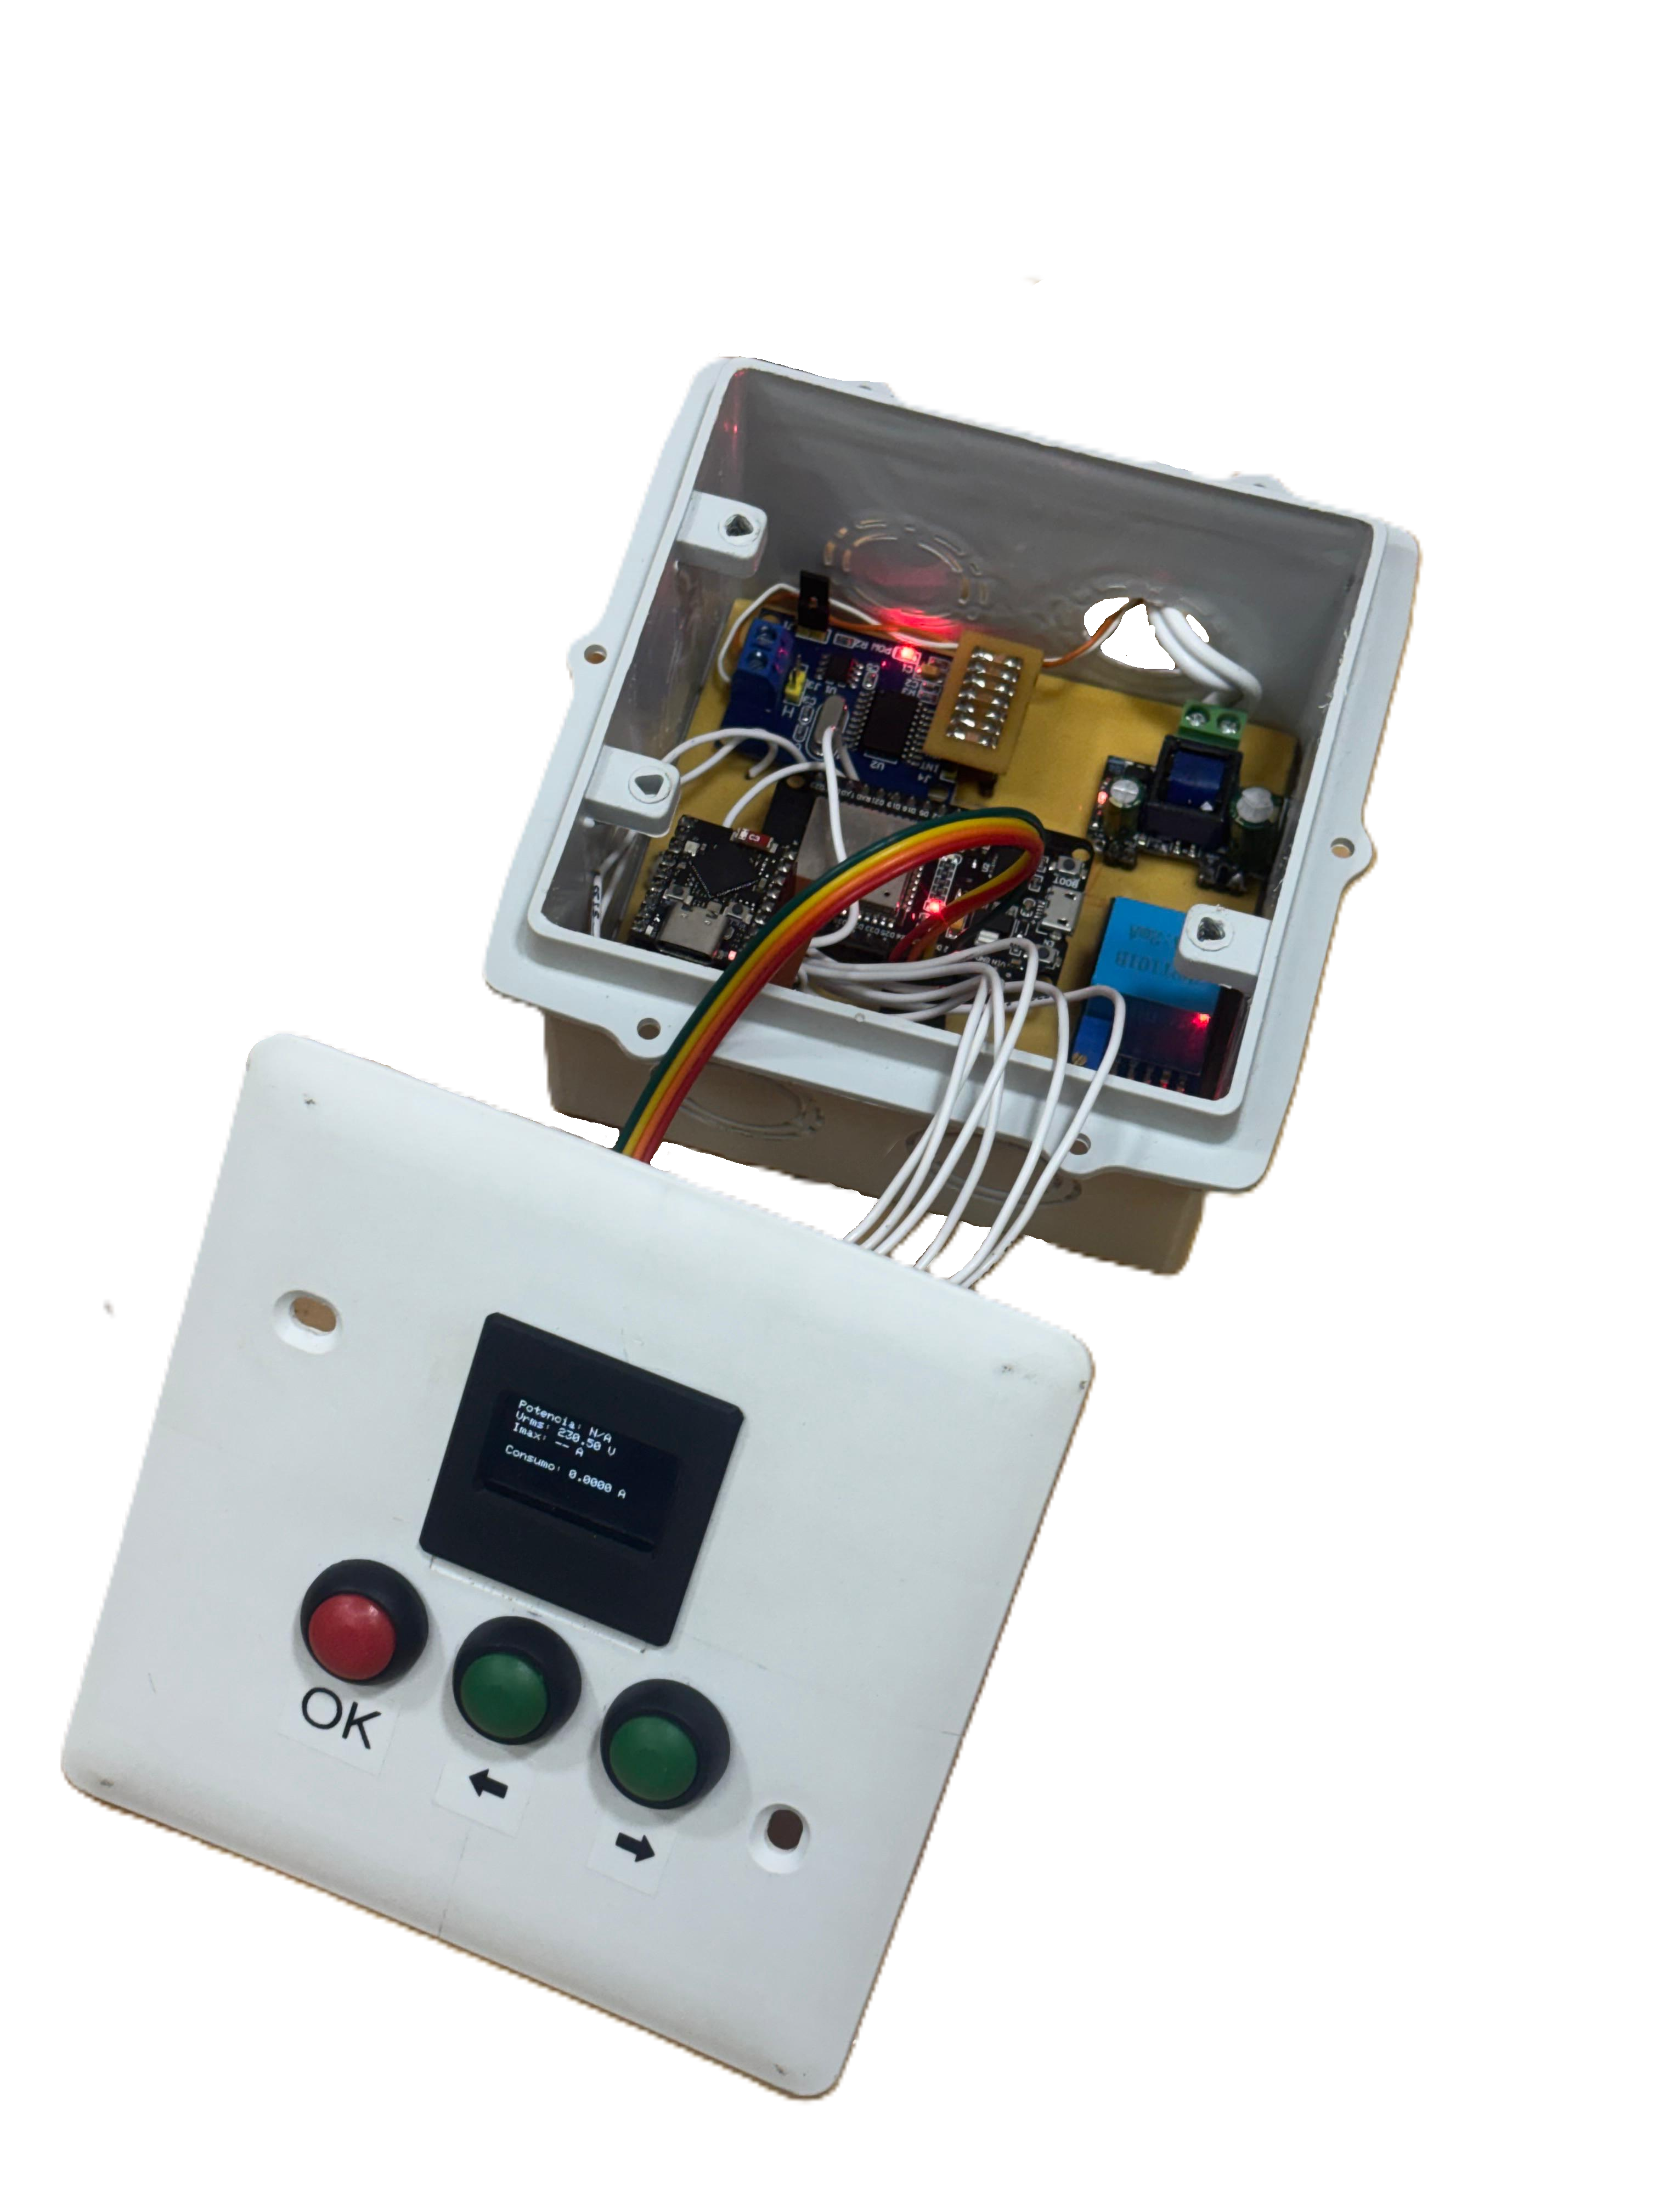
\includegraphics[width=0.35\textwidth]{imagenes/ac.png}
    \caption{Hardware desarrollado para el Agente de Carga(AC)}
    \label{img:ac}
\end{figure}
\section{Firmware}
